% ============================================================================
%  Photon ID Meeting — Cell-Level Shower Shape Corrections
%  Marta Fernandes da Silva, 10 March 2026
% ============================================================================
\documentclass[aspectratio=169,10pt]{beamer}

% --- Theme & colours --------------------------------------------------------
\usetheme{Madrid}
\usecolortheme{default}
\definecolor{atlasblue}{RGB}{0,73,135}
\setbeamercolor{structure}{fg=atlasblue}
\setbeamercolor{frametitle}{bg=atlasblue!10, fg=atlasblue}
\setbeamercolor{title}{fg=white, bg=atlasblue}
\setbeamercolor{block title}{bg=atlasblue, fg=white}
\setbeamercolor{block body}{bg=atlasblue!5}
\setbeamercolor{item}{fg=atlasblue}
\setbeamertemplate{navigation symbols}{}
\setbeamertemplate{footline}{%
  \leavevmode\hbox{%
    \begin{beamercolorbox}[wd=.33\paperwidth,ht=2.5ex,dp=1ex,center]{author in head/foot}%
      \usebeamerfont{author in head/foot}\insertshortauthor
    \end{beamercolorbox}%
    \begin{beamercolorbox}[wd=.34\paperwidth,ht=2.5ex,dp=1ex,center]{title in head/foot}%
      \usebeamerfont{title in head/foot}\insertshorttitle
    \end{beamercolorbox}%
    \begin{beamercolorbox}[wd=.33\paperwidth,ht=2.5ex,dp=1ex,right]{date in head/foot}%
      \usebeamerfont{date in head/foot}\insertshortdate{}\hspace*{2em}
      \insertframenumber{}/\inserttotalframenumber\hspace*{2ex}
    \end{beamercolorbox}}%
  \vskip0pt%
}

% --- Packages ---------------------------------------------------------------
\usepackage[utf8]{inputenc}
\usepackage[T1]{fontenc}
\usepackage{amsmath,amssymb}
\usepackage{graphicx}
\usepackage{booktabs}
\usepackage{tikz}
\usetikzlibrary{decorations.pathreplacing}
\usepackage{siunitx}
\usepackage{appendixnumberbeamer}

% --- Graphics path ----------------------------------------------------------
\graphicspath{
  {../output/closure_test_5pct/}
  {../output/closure_test_3pct/}
  {../output/closure_test_1pct/}
  {../output/plots/}
}

% --- Title info -------------------------------------------------------------
\title[Cell-Level Shower Shape Corrections]{%
  Cell-Level Shower Shape Corrections\\[2pt]
  for Photon ID in MC23e}
\author[M.~Fernandes da Silva]{Marta Fernandes da Silva}
\institute{LIP / ATLAS}
\date{Photon ID Meeting — 10 March 2026}

% ============================================================================
\begin{document}
% ============================================================================

% --- Slide 1: Title ---------------------------------------------------------
{
\setbeamertemplate{footline}{}
\begin{frame}
  \titlepage
  \vfill
  \centering
  {\small\color{gray} ATLAS Internal}
\end{frame}
}

% --- Slide 2: Outline -------------------------------------------------------
\begin{frame}{Outline}
  \tableofcontents
\end{frame}

% ============================================================================
\section{Motivation \& Context}
% ============================================================================

% --- Slide 3: Photon ID & Shower Shapes ------------------------------------
\begin{frame}{Photon Identification \& Shower Shapes}

\begin{columns}[T]
\begin{column}{0.55\textwidth}
  \textbf{Photon identification in ATLAS} uses a cut-based approach
  on calorimeter and tracking variables:
  \begin{itemize}
    \item \textbf{Loose} and \textbf{Tight} working points defined by
          rectangular cuts on \emph{shower shape variables}
    \item Shower shapes characterise the \textbf{lateral and longitudinal
          energy profile} of the electromagnetic shower
    \item Key discriminants in the \textbf{second EM sampling layer}
          (Layer~2): $R_\eta$, $R_\phi$, $w_{\eta\,2}$
    \item Also used: Layer~1 strip variables ($w_{s\,3}$, $w_{s\,\text{tot}}$,
          $F_\text{side}$, $\Delta E$, $E_\text{ratio}$), hadronic leakage
  \end{itemize}
  \vspace{4pt}
  Accurate modelling of shower shapes in MC is \textbf{essential} for
  measuring photon ID efficiency via data-driven methods (e.g.\ tag-and-probe
  with $Z\to\ell\ell\gamma$).
\end{column}
\begin{column}{0.42\textwidth}
  % Placeholder for calorimeter diagram from Francisco's report
  % Uncomment and adjust path after extracting figure:
  % \includegraphics[width=\textwidth]{fig_calorimeter.pdf}
  \begin{center}
  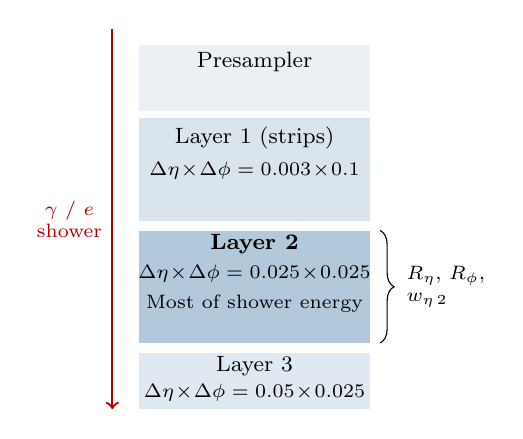
\begin{tikzpicture}[scale=0.42]
    % Simplified EM calorimeter layer schematic
    \fill[atlasblue!8] (0,3.5) rectangle (7,5.5);
    \node[font=\footnotesize] at (3.5,5.0) {Presampler};
    \fill[atlasblue!15] (0,0.2) rectangle (7,3.3);
    \node[font=\footnotesize] at (3.5,2.7) {Layer 1 (strips)};
    \node[font=\scriptsize] at (3.5,1.7) {$\Delta\eta\!\times\!\Delta\phi = 0.003\!\times\!0.1$};
    \fill[atlasblue!30] (0,-3.5) rectangle (7,-0.1);
    \node[font=\footnotesize\bfseries] at (3.5,-0.5) {Layer 2};
    \node[font=\scriptsize] at (3.5,-1.4) {$\Delta\eta\!\times\!\Delta\phi = 0.025\!\times\!0.025$};
    \node[font=\scriptsize] at (3.5,-2.3) {Most of shower energy};
    \fill[atlasblue!12] (0,-5.5) rectangle (7,-3.8);
    \node[font=\footnotesize] at (3.5,-4.2) {Layer 3};
    \node[font=\scriptsize] at (3.5,-5.0) {$\Delta\eta\!\times\!\Delta\phi = 0.05\!\times\!0.025$};
    % arrow
    \draw[->,thick,red!70!black] (-0.8,6.0) -- (-0.8,-5.5)
      node[midway,left,font=\scriptsize,align=center] {$\gamma$ / $e$\\shower};
    % braces
    \draw[decorate,decoration={brace,mirror,amplitude=5pt}]
      (7.3,-3.5) -- (7.3,-0.1)
      node[midway,right=6pt,font=\scriptsize,align=left] {$R_\eta$, $R_\phi$,\\$w_{\eta\,2}$};
  \end{tikzpicture}
  \end{center}
\end{column}
\end{columns}
\end{frame}

% --- Slide 4: Fudge Factors & Motivation -----------------------------------
\begin{frame}{Current Corrections \& Motivation for Cell-Level Approach}

\begin{columns}[T]
\begin{column}{0.48\textwidth}
  \textbf{Current approach: fudge factors}
  \begin{itemize}
    \item Data--MC differences in shower shapes corrected by
          per-variable \textbf{shifts and smearings}
    \item Derived from $Z\to ee$ control samples, applied to MC
    \item Each variable corrected \emph{independently}
  \end{itemize}
  \vspace{4pt}
  \textbf{Limitations:}
  \begin{itemize}
    \item Does \textbf{not} preserve correlations between variables
    \item Corrections derived at distribution level, not event level
    \item Not suitable for ML-based ID (CNN/GNN) that uses
          cell-level inputs directly
    \item Must be re-derived for every new variable
  \end{itemize}
\end{column}
\begin{column}{0.48\textwidth}
  \textbf{Cell-level approach:}
  \begin{itemize}
    \item Correct individual \textbf{cell energies} in the EM
          calorimeter cluster
    \item Recompute \emph{all} shower shapes from corrected cells
    \item Inter-variable correlations preserved
          \textbf{by construction}
    \item Any new variable automatically benefits
    \item Enables consistent input for both cut-based and ML-based ID
  \end{itemize}
  \vspace{4pt}
  \textbf{Pioneered for Run~2} in ATL-COM-PHYS-2021-640\\
  (F.~Caetano et al.) — applied to Layer~2 cells using
  $Z\to\ell\ell\gamma$ matched data--MC ntuples.
\end{column}
\end{columns}
\end{frame}

% --- Slide 5: Project Goal -------------------------------------------------
\begin{frame}{Project Goal}

\begin{block}{Objective}
Continue and extend the cell-level shower shape correction studies
for \textbf{Run~3 conditions} (MC23), building on the Run~2 method
developed in ATL-COM-PHYS-2021-640.
\end{block}
\vspace{6pt}

\textbf{Previous work} (Run~2, F.~Caetano et al.):
\begin{itemize}
  \item Cell-energy reweighting applied to \textbf{Layer~2} of the EM calorimeter
  \item Used matched data--MC event pairs from $Z\to\ell\ell\gamma$
  \item Two correction methods studied: flat shift and energy-dependent (TProfile)
  \item Demonstrated improved data--MC agreement for $R_\eta$, $R_\phi$,
        $w_{\eta\,2}$
\end{itemize}
\vspace{6pt}

\textbf{This work — scope:}
\begin{enumerate}
  \item \textbf{Validate} the method with Run~3 MC (MC23e) via closure tests
  \item \textbf{Apply} corrections to real Run~3 data using DAOD\_EGAM3 ntuples
  \item \textbf{Extend} the approach to \textbf{Layers~1 and~3} of the EM calorimeter
        (strip and back layers)
\end{enumerate}
\end{frame}

% ============================================================================
\section{Shower Shape Variables}
% ============================================================================

% --- Slide 5: Shower Shape Variables ----------------------------------------
\begin{frame}{Shower Shape Variables}
\begin{columns}[T]
\begin{column}{0.45\textwidth}
  \textbf{Three key discriminants:}
  \vspace{4pt}

  \begin{align*}
    R_\eta &= \frac{E(3\!\times\!7)}{E(7\!\times\!7)}
    \\[6pt]
    R_\phi &= \frac{E(3\!\times\!3)}{E(3\!\times\!7)}
    \\[6pt]
    w_{\eta\,2} &= \sqrt{
      \frac{\sum E_i\,\eta_i^2}{\sum E_i}
      - \left(\frac{\sum E_i\,\eta_i}{\sum E_i}\right)^{\!2}
    }
  \end{align*}
  \vspace{4pt}

  {\small $E(m\!\times\!n)$: energy in $m\,(\eta)\times n\,(\phi)$
  sub-window.\\ $w_{\eta\,2}$ computed in $3\!\times\!5$ window.}
\end{column}
\begin{column}{0.52\textwidth}
  \centering
  % TikZ diagram of 7x11 cell grid with sub-windows
  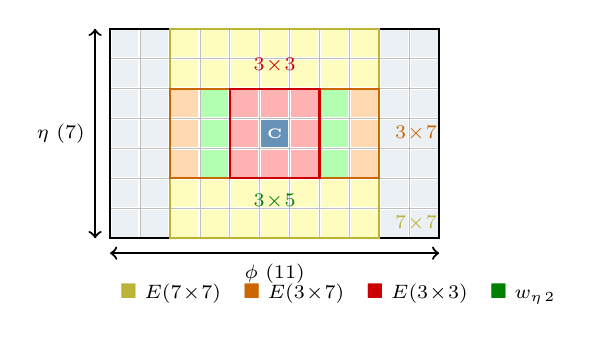
\begin{tikzpicture}[scale=0.38, every node/.style={font=\tiny}]
    % Full 7x11 grid (7 eta rows, 11 phi cols)
    \foreach \r in {0,...,6} {
      \foreach \c in {0,...,10} {
        \fill[atlasblue!8] (\c+0.05,\r+0.05) rectangle (\c+0.95,\r+0.95);
      }
    }
    % 7x7 window (all 7 rows, cols 2-8) — lightest highlight
    \foreach \r in {0,...,6} {
      \foreach \c in {2,...,8} {
        \fill[yellow!25] (\c+0.05,\r+0.05) rectangle (\c+0.95,\r+0.95);
      }
    }
    % 3x7 window (rows 2-4, cols 2-8)
    \foreach \r in {2,...,4} {
      \foreach \c in {2,...,8} {
        \fill[orange!30] (\c+0.05,\r+0.05) rectangle (\c+0.95,\r+0.95);
      }
    }
    % 3x5 window for weta2 (rows 2-4, cols 3-7)
    \foreach \r in {2,...,4} {
      \foreach \c in {3,...,7} {
        \fill[green!30] (\c+0.05,\r+0.05) rectangle (\c+0.95,\r+0.95);
      }
    }
    % 3x3 window (rows 2-4, cols 4-6)
    \foreach \r in {2,...,4} {
      \foreach \c in {4,...,6} {
        \fill[red!30] (\c+0.05,\r+0.05) rectangle (\c+0.95,\r+0.95);
      }
    }
    % Central cell highlight
    \fill[atlasblue!60] (5+0.05,3+0.05) rectangle (5+0.95,3+0.95);
    \node[white,font=\tiny\bfseries] at (5.5,3.5) {C};
    % Grid lines
    \draw[gray!50,very thin] (0,0) grid (11,7);
    % Outer border
    \draw[thick] (0,0) rectangle (11,7);
    % Sub-window borders
    \draw[yellow!70!black,thick] (2,0) rectangle (9,7);
    \draw[orange!80!black,thick] (2,2) rectangle (9,5);
    \draw[red!80!black,thick] (4,2) rectangle (7,5);
    % Labels
    \node[yellow!70!black,anchor=west,font=\scriptsize\bfseries]
      at (9.2,0.5) {$7\!\times\!7$};
    \node[orange!80!black,anchor=west,font=\scriptsize\bfseries]
      at (9.2,3.5) {$3\!\times\!7$};
    \node[red!80!black,anchor=south,font=\scriptsize\bfseries]
      at (5.5,5.2) {$3\!\times\!3$};
    \node[green!50!black,anchor=north,font=\scriptsize\bfseries]
      at (5.5,1.8) {$3\!\times\!5$};
    % Axes
    \draw[<->,thick] (-0.5,0) -- (-0.5,7)
      node[midway,left,font=\scriptsize] {$\eta$ (7)};
    \draw[<->,thick] (0,-0.5) -- (11,-0.5)
      node[midway,below,font=\scriptsize] {$\phi$ (11)};
    % Legend
    \node[anchor=north west,font=\scriptsize,align=left] at (0,-1.2) {%
      \textcolor{yellow!70!black}{$\blacksquare$}~$E(7\!\times\!7)$\quad
      \textcolor{orange!80!black}{$\blacksquare$}~$E(3\!\times\!7)$\quad
      \textcolor{red!80!black}{$\blacksquare$}~$E(3\!\times\!3)$\quad
      \textcolor{green!50!black}{$\blacksquare$}~$w_{\eta\,2}$
    };
  \end{tikzpicture}
\end{column}
\end{columns}
\end{frame}

% ============================================================================
\section{Cell-Energy Reweighting Method}
% ============================================================================

% --- Slide 6: Method Overview -----------------------------------------------
\begin{frame}{Cell-Energy Reweighting: Overview}

\begin{enumerate}
  \item \textbf{Compute cell energy fractions} from the $7\!\times\!11$ cluster:
  \[
    f_k \;=\; \frac{e_k}{E_\text{tot}}
    \;=\; \frac{e_k}{\displaystyle\sum_{j=1}^{77} e_j}
    \qquad (k = 1,\ldots,77)
  \]

  \item \textbf{Derive correction} by comparing data and MC fractions
        cell-by-cell, in each of 14~$|\eta|$ bins

  \item \textbf{Apply correction} to MC fractions:
  $\quad f_k^\text{corr} = f_k^\text{MC} + \text{correction}_k$

  \item \textbf{Reconstruct cell energies} with energy conservation:
  \[
    e_k^\text{corr} \;=\;
    \frac{f_k^\text{corr}}{\displaystyle\sum_j f_j^\text{corr}}
    \;\times\; E_\text{tot}
  \]

  \item \textbf{Recompute all shower shapes} from the corrected cell energies
\end{enumerate}

\vspace{4pt}
\centering
{\small\color{atlasblue} Two methods differ in step~2: how the correction is parameterised}
\end{frame}

% --- Slide 7: Method 1 vs Method 2 -----------------------------------------
\begin{frame}{Correction Methods}
\begin{columns}[T]
\begin{column}{0.48\textwidth}
  \begin{block}{Method 1: Flat Shift}
    One number per cell per $|\eta|$ bin:
    \[
      \Delta_k = \langle f_k^\text{data}\rangle
              - \langle f_k^\text{MC}\rangle
    \]
    Applied as:
    \[
      f_k^\text{corr} = f_k^\text{MC} + \Delta_k
    \]
    \vspace{2pt}
    \begin{itemize}
      \item Simple, robust
      \item Ignores energy dependence of correction
    \end{itemize}
  \end{block}
\end{column}
\begin{column}{0.48\textwidth}
  \begin{block}{Method 2: TProfile (Energy-Dependent)}
    Correction varies with cell fraction:
    \[
      \alpha_k(f) = \bigl\langle f_k^\text{data}
        - f_k^\text{MC}\bigr\rangle\Big|_{f_k^\text{MC}=f}
    \]
    Applied via interpolation:
    \[
      f_k^\text{corr} = f_k^\text{MC}
        + \alpha_k\!\bigl(f_k^\text{MC}\bigr)
    \]
    \vspace{2pt}
    \begin{itemize}
      \item Captures non-linear effects
      \item 1078 profile histograms\\
            {\small ($77~\text{cells}\times 14~|\eta|~\text{bins}$)}
    \end{itemize}
  \end{block}
\end{column}
\end{columns}
\vspace{8pt}
\centering
{\small Following ATL-COM-PHYS-2021-640, Sections~5.1 and~5.2
(F.~Caetano et al.)}
\end{frame}

% ============================================================================
\section{Closure Test}
% ============================================================================

% --- Slide 9: Closure Test Setup -------------------------------------------
\begin{frame}{Closure Test: Setup \& Inputs}

\textbf{Goal}: validate the correction procedure in a controlled environment
where the ``truth'' is known by construction.

\vspace{4pt}
\begin{columns}[T]
\begin{column}{0.48\textwidth}
  \textbf{Monte Carlo sample}
  \begin{itemize}
    \item MC23e $Z\to ee\gamma$, DSID~700770
    \item Sherpa~2.2.14, Run~3 simulation
    \item $\sim$9.6\,M events total
    \item $\sim$7.8\,M pass quality selection (81\%)
  \end{itemize}
  \vspace{4pt}
  \textbf{Ntuple production}
  \begin{itemize}
    \item NTupleMaker package (Athena 25.0.40)
    \item Layer~2 cell energies stored as vector of
          77 doubles ($7\!\times\!11$ cluster)
    \item Cluster barycentre $\eta_2$ for binning
  \end{itemize}
\end{column}
\begin{column}{0.48\textwidth}
  \textbf{$|\eta|$ binning} — 14~bins, standard ATLAS
  EM calorimeter segmentation:
  {\small
  \[
    [0,0.2),\; [0.2,0.4),\; \ldots\; [1.3,1.37)
  \]
  \[
    [1.52,1.6),\; \ldots\; [2.2,2.4)
  \]
  }
  Crack region $1.37 < |\eta| < 1.52$ excluded.
  \vspace{4pt}

  \textbf{Quality selection}
  \begin{itemize}
    \item \textbf{Central cell dominance}: cell~$(3,5)$ must
          carry highest energy fraction
    \item \textbf{Negative energy clamping}: cells with $e_k < 0$
          (noise) set to zero
  \end{itemize}
\end{column}
\end{columns}
\end{frame}

% --- Slide 10: Closure Test Design ------------------------------------------
\begin{frame}{Closure Test: Distortion Model}

\textbf{Goal}: validate the correction in a controlled environment where the
``truth'' is known by construction.

\vspace{4pt}
\begin{columns}[T]
\begin{column}{0.55\textwidth}
  \textbf{Distortion model} — generate pseudo-data from MC:
  \[
    e'_k = e_k \cdot \bigl(1 + \delta\cdot b_k + \varepsilon_k\bigr)
  \]
  \begin{itemize}
    \item $\delta$: systematic distortion level (1\%, 3\%, 5\%)
    \item $b_k$: fixed bias pattern (narrowing)
    \item $\varepsilon_k \sim \mathcal{N}(0,\,\delta/2)$: stochastic noise
    \item Total cluster energy conserved by rescaling
  \end{itemize}
  \vspace{4pt}
  \textbf{Quality selection:}
  \begin{itemize}
    \item Central cell must have highest energy fraction
    \item Negative cell energies clamped to zero
  \end{itemize}
\end{column}
\begin{column}{0.42\textwidth}
  \centering
  \textbf{Bias pattern $b_k$}\\[4pt]
  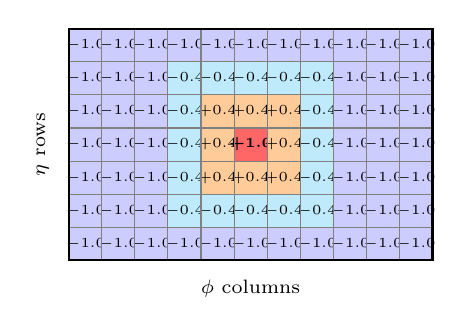
\begin{tikzpicture}[scale=0.42, every node/.style={font=\tiny}]
    % Draw 7x11 grid with bias pattern colouring
    \foreach \r in {0,...,6} {
      \foreach \c in {0,...,10} {
        % Compute Chebyshev distance from centre (3,5)
        \pgfmathtruncatemacro{\dr}{abs(\r - 3)}
        \pgfmathtruncatemacro{\dc}{abs(\c - 5)}
        \pgfmathtruncatemacro{\dist}{max(\dr,\dc)}
        \ifnum\dist=0
          \fill[red!60] (\c,\r) rectangle (\c+1,\r+1);
          \node at (\c+0.5,\r+0.5) {\textbf{+1.0}};
        \else\ifnum\dist=1
          \fill[orange!40] (\c,\r) rectangle (\c+1,\r+1);
          \node at (\c+0.5,\r+0.5) {+0.4};
        \else\ifnum\dist=2
          \fill[cyan!25] (\c,\r) rectangle (\c+1,\r+1);
          \node at (\c+0.5,\r+0.5) {$-$0.4};
        \else
          \fill[blue!20] (\c,\r) rectangle (\c+1,\r+1);
          \node at (\c+0.5,\r+0.5) {$-$1.0};
        \fi\fi\fi
      }
    }
    \draw[gray,thin] (0,0) grid (11,7);
    \draw[thick] (0,0) rectangle (11,7);
    % Labels
    \node[font=\scriptsize,below] at (5.5,-0.3) {$\phi$ columns};
    \node[font=\scriptsize,rotate=90,above] at (-0.3,3.5) {$\eta$ rows};
  \end{tikzpicture}
  \\[4pt]
  {\scriptsize Mimics narrower showers (data-like):\\
  enhance core, suppress tails}
\end{column}
\end{columns}
\end{frame}

% --- Slide 9: Validation ---------------------------------------------------
\begin{frame}{Validation: Shower Shape Recomputation}

Before running the closure test, verified that shower shapes computed
from the $7\!\times\!11$ cell energies \textbf{match the stored values}
in the ntuples.

\vspace{6pt}
\begin{columns}[c]
\begin{column}{0.32\textwidth}
  \centering
  \includegraphics[width=\textwidth]{reta_Zeeg.pdf}\\
  {\small $R_\eta$ — $Z\to ee\gamma$}
\end{column}
\begin{column}{0.32\textwidth}
  \centering
  \includegraphics[width=\textwidth]{rphi_Zeeg.pdf}\\
  {\small $R_\phi$ — $Z\to ee\gamma$}
\end{column}
\begin{column}{0.32\textwidth}
  \centering
  \includegraphics[width=\textwidth]{weta2_Zeeg.pdf}\\
  {\small $w_{\eta\,2}$ — $Z\to ee\gamma$}
\end{column}
\end{columns}

\vspace{6pt}
\centering
{\small Excellent agreement validates the cell-energy $\to$ shower-shape
computation pipeline.\\
$w_{\eta\,2}$ uses relative cell positions
($\eta_i \in \{0,\,\Delta\eta,\,2\Delta\eta\}$) — valid since
$w_{\eta\,2}$ is translation-invariant.}
\end{frame}

% ============================================================================
\section{Results}
% ============================================================================

% --- Slide 10: Closure — Central Barrel 5% ---------------------------------
\begin{frame}{Closure Results: Central Barrel ($\delta = 5\%$)}

$|\eta|\in[0.00,\,0.20)$ — 5\% distortion level — full statistics
(9.6\,M events)

\vspace{4pt}
\begin{columns}[c]
\begin{column}{0.32\textwidth}
  \centering
  \includegraphics[page=1,width=\textwidth]{closure_reta.pdf}\\
  {\small $R_\eta$}
\end{column}
\begin{column}{0.32\textwidth}
  \centering
  \includegraphics[page=1,width=\textwidth]{closure_rphi.pdf}\\
  {\small $R_\phi$}
\end{column}
\begin{column}{0.32\textwidth}
  \centering
  \includegraphics[page=1,width=\textwidth]{closure_weta2.pdf}\\
  {\small $w_{\eta\,2}$}
\end{column}
\end{columns}

\vspace{6pt}
\centering
{\small
  \textcolor{black!70}{$\bullet$}~Pseudo-data\quad
  \textcolor{red}{---}~MC (uncorrected)\quad
  \textcolor{green!60!black}{- -}~Method~1\quad
  \textcolor{blue}{---}~Method~2\\[2pt]
  Method~2 brings ratio to within $\sim$1\% of unity across the full range.
}
\end{frame}

% --- Slide 11: Distortion Level Scan ----------------------------------------
\begin{frame}{Distortion Level Comparison ($R_\eta$, Central Barrel)}

$|\eta|\in[0.00,\,0.20)$ — comparing 1\%, 3\%, and 5\% distortion levels

\vspace{4pt}
\begin{columns}[c]
\begin{column}{0.32\textwidth}
  \centering
  \includegraphics[page=1,width=\textwidth]{../output/closure_test_1pct/closure_reta.pdf}\\
  {\small $\delta = 1\%$}
\end{column}
\begin{column}{0.32\textwidth}
  \centering
  \includegraphics[page=1,width=\textwidth]{../output/closure_test_3pct/closure_reta.pdf}\\
  {\small $\delta = 3\%$}
\end{column}
\begin{column}{0.32\textwidth}
  \centering
  \includegraphics[page=1,width=\textwidth]{../output/closure_test_5pct/closure_reta.pdf}\\
  {\small $\delta = 5\%$}
\end{column}
\end{columns}

\vspace{6pt}
\centering
{\small
  At 1\%: distributions nearly indistinguishable.
  At 5\%: discrepancy clearly visible; Method~2 superiority most evident.\\[2pt]
  Correction performance \textbf{scales well} with distortion magnitude.
}
\end{frame}

% --- Slide 13: Chi2 Summary ------------------------------------------------
\begin{frame}{$\chi^2/n_\text{df}$ Summary ($\delta = 5\%$)}

\centering
\small
\begin{tabular}{
  c
  c@{\hskip 6pt}c@{\hskip 6pt}c
  c@{\hskip 6pt}c@{\hskip 6pt}c
  c@{\hskip 6pt}c@{\hskip 6pt}c
}
\toprule
& \multicolumn{3}{c}{$R_\eta$}
& \multicolumn{3}{c}{$R_\phi$}
& \multicolumn{3}{c}{$w_{\eta\,2}$} \\
\cmidrule(lr){2-4}\cmidrule(lr){5-7}\cmidrule(lr){8-10}
$|\eta|$ bin & MC & M1 & \textbf{M2}
             & MC & M1 & \textbf{M2}
             & MC & M1 & \textbf{M2} \\
\midrule
$[0.0,\,0.2)$   & 0.0059 & 0.0046 & \textbf{0.0005} & 0.0052 & 0.0014 & \textbf{0.0006} & 0.0014 & 0.0005 & \textbf{0.0003} \\
$[0.4,\,0.6)$   & 0.0063 & 0.0037 & \textbf{0.0005} & 0.0054 & 0.0015 & \textbf{0.0006} & 0.0018 & 0.0007 & \textbf{0.0004} \\
$[0.8,\,1.0)$   & 0.0079 & 0.0028 & \textbf{0.0006} & 0.0052 & 0.0021 & \textbf{0.0003} & 0.0022 & 0.0009 & \textbf{0.0006} \\
$[1.3,\,1.37)$  & 0.0085 & 0.0026 & \textbf{0.0008} & 0.0051 & 0.0026 & \textbf{0.0006} & 0.0023 & 0.0010 & \textbf{0.0006} \\
$[1.52,\,1.6)$  & 0.0078 & 0.0062 & \textbf{0.0004} & 0.0022 & 0.0014 & \textbf{0.0002} & 0.0011 & 0.0016 & \textbf{0.0007} \\
$[1.8,\,2.0)$   & 0.0139 & 0.0033 & \textbf{0.0010} & 0.0087 & 0.0038 & \textbf{0.0004} & 0.0032 & 0.0008 & \textbf{0.0007} \\
$[2.2,\,2.4)$   & 0.0192 & 0.0035 & \textbf{0.0010} & 0.0118 & 0.0034 & \textbf{0.0005} & 0.0040 & 0.0010 & \textbf{0.0008} \\
\bottomrule
\end{tabular}

\vspace{8pt}
\begin{columns}[T]
\begin{column}{0.48\textwidth}
  \textbf{Method~1} (flat shift):
  \begin{itemize}
    \item 50--80\% $\chi^2$ reduction
  \end{itemize}
\end{column}
\begin{column}{0.48\textwidth}
  \textbf{Method~2} (TProfile):
  \begin{itemize}
    \item \textbf{90--95\% $\chi^2$ reduction}
    \item Consistent across all $|\eta|$ bins and all 3 variables
  \end{itemize}
\end{column}
\end{columns}
\end{frame}

% ============================================================================
\section{Conclusions \& Next Steps}
% ============================================================================

% --- Slide 15: Conclusions & Next Steps ------------------------------------
\begin{frame}{Conclusions \& Next Steps}

\textbf{Conclusions:}
\begin{itemize}
  \item Cell-energy reweighting method successfully \textbf{validated} for
        Run~3 MC (MC23e) via closure tests
  \item Tested at 3~distortion levels (1\%, 3\%, 5\%) across
        13~populated $|\eta|$ bins
  \item \textbf{Method~2} (energy-dependent TProfile) achieves
        \textbf{90--95\%} $\chi^2/n_\text{df}$ reduction —
        consistently outperforms flat shift (Method~1: 50--80\%)
  \item Correction is \textbf{uniform} across all $|\eta|$ bins and all
        3 shower shape variables ($R_\eta$, $R_\phi$, $w_{\eta\,2}$)
\end{itemize}

\vspace{6pt}
\textbf{Next steps:}
\begin{enumerate}
  \item \textbf{Data--MC comparison} — apply corrections to real Run~3 data
    \begin{itemize}
      \item DAOD\_EGAM3 ntuples produced
            (data24 run~473235 + MC23e DSID~700770)
      \item Analysis pipeline implemented, pending execution
    \end{itemize}
  \item \textbf{Conversion-type binning}
        (derive separate corrections for unconverted / converted photons)
  \item \textbf{Extend to Layers~1 and~3}
        (requires new NTupleMaker branches for L1/L3 cell energies)
  \item Study impact on \textbf{photon ID efficiency} (tight working point)
\end{enumerate}
\end{frame}

% ============================================================================
% BACKUP SLIDES
% ============================================================================
\appendix
\begin{frame}[noframenumbering]
  \centering
  \Huge\bfseries\color{atlasblue}
  Backup
\end{frame}

% --- Backup: Key Adaptations from Reference --------------------------------
\begin{frame}[noframenumbering]{Key Adaptations from Reference Method}

\small
Differences from ATL-COM-PHYS-2021-640 (Run~2 implementation):

\vspace{4pt}
\begin{tabular}{lll}
\toprule
\textbf{Aspect} & \textbf{Reference (Run~2)} & \textbf{This work (MC23e)} \\
\midrule
Input format     & Matched data--MC pairs     & Unmatched MC \\
Pre-selection    & Tight ID + isolation       & Central cell + energy clamping \\
$w_{\eta\,2}$ coords & Absolute cell $\eta$  & Relative positions
                       ($\Delta\eta\!=\!0.025$) \\
Conv.\ binning   & Inc / UnConv / Conv        & Inclusive only$^\dagger$ \\
Precision        & \texttt{float}             & \texttt{double} \\
\bottomrule
\end{tabular}

\vspace{8pt}
\begin{itemize}
  \item Central cell cut removes mis-centred/pathological clusters
  \item Negative energy clamping prevents unphysical fractions ($f_k > 1$
        or $f_k < 0$)
  \item Relative $\eta$ valid: $w_{\eta\,2}$ is a second central moment
        (translation-invariant)
  \item[$^\dagger$] Conversion-type binning planned for data application
\end{itemize}
\end{frame}

% --- Backup: Forward Endcap ------------------------------------------------
\begin{frame}[noframenumbering]{Closure Results: Forward Endcap ($\delta = 5\%$)}

$|\eta|\in[2.20,\,2.40)$ — demonstrates method works at high pseudorapidity

\vspace{4pt}
\begin{columns}[c]
\begin{column}{0.32\textwidth}
  \centering
  \includegraphics[page=13,width=\textwidth]{closure_reta.pdf}\\
  {\small $R_\eta$}
\end{column}
\begin{column}{0.32\textwidth}
  \centering
  \includegraphics[page=13,width=\textwidth]{closure_rphi.pdf}\\
  {\small $R_\phi$}
\end{column}
\begin{column}{0.32\textwidth}
  \centering
  \includegraphics[page=13,width=\textwidth]{closure_weta2.pdf}\\
  {\small $w_{\eta\,2}$}
\end{column}
\end{columns}

\vspace{6pt}
\centering
{\small
  Uncorrected $\chi^2/n_\text{df}$ is larger at forward $|\eta|$
  (different detector geometry),\\
  but Method~2 still achieves $\sim$20$\times$ reduction.
}
\end{frame}

% --- Backup: Full chi2 table 5% --------------------------------------------
\begin{frame}[noframenumbering]{Full $\chi^2/n_\text{df}$: 5\% Distortion}
\centering
\scriptsize
\begin{tabular}{
  c
  c@{\hskip 4pt}c@{\hskip 4pt}c
  c@{\hskip 4pt}c@{\hskip 4pt}c
  c@{\hskip 4pt}c@{\hskip 4pt}c
}
\toprule
& \multicolumn{3}{c}{$R_\eta$}
& \multicolumn{3}{c}{$R_\phi$}
& \multicolumn{3}{c}{$w_{\eta\,2}$} \\
\cmidrule(lr){2-4}\cmidrule(lr){5-7}\cmidrule(lr){8-10}
{$|\eta|$ bin} & {MC} & {M1} & {M2} & {MC} & {M1} & {M2} & {MC} & {M1} & {M2} \\
\midrule
0  & 0.0059 & 0.0046 & 0.0005 & 0.0052 & 0.0014 & 0.0006 & 0.0014 & 0.0005 & 0.0003 \\
1  & 0.0064 & 0.0037 & 0.0005 & 0.0053 & 0.0014 & 0.0006 & 0.0017 & 0.0007 & 0.0004 \\
2  & 0.0063 & 0.0037 & 0.0005 & 0.0054 & 0.0015 & 0.0006 & 0.0018 & 0.0007 & 0.0004 \\
3  & 0.0062 & 0.0035 & 0.0004 & 0.0051 & 0.0014 & 0.0005 & 0.0018 & 0.0008 & 0.0004 \\
4  & 0.0079 & 0.0028 & 0.0006 & 0.0052 & 0.0021 & 0.0003 & 0.0022 & 0.0009 & 0.0006 \\
5  & 0.0077 & 0.0027 & 0.0005 & 0.0050 & 0.0016 & 0.0003 & 0.0022 & 0.0010 & 0.0006 \\
6  & 0.0074 & 0.0027 & 0.0005 & 0.0050 & 0.0016 & 0.0004 & 0.0022 & 0.0011 & 0.0007 \\
7  & 0.0085 & 0.0026 & 0.0008 & 0.0051 & 0.0026 & 0.0006 & 0.0023 & 0.0010 & 0.0006 \\
9  & 0.0078 & 0.0062 & 0.0004 & 0.0022 & 0.0014 & 0.0002 & 0.0011 & 0.0016 & 0.0007 \\
10 & 0.0090 & 0.0038 & 0.0004 & 0.0049 & 0.0019 & 0.0003 & 0.0019 & 0.0011 & 0.0007 \\
11 & 0.0139 & 0.0033 & 0.0010 & 0.0087 & 0.0038 & 0.0004 & 0.0032 & 0.0008 & 0.0007 \\
12 & 0.0169 & 0.0032 & 0.0010 & 0.0106 & 0.0034 & 0.0005 & 0.0036 & 0.0008 & 0.0007 \\
13 & 0.0192 & 0.0035 & 0.0010 & 0.0118 & 0.0034 & 0.0005 & 0.0040 & 0.0010 & 0.0008 \\
\bottomrule
\end{tabular}
\end{frame}

% --- Backup: Full chi2 table 3% --------------------------------------------
\begin{frame}[noframenumbering]{Full $\chi^2/n_\text{df}$: 3\% Distortion}
\centering
\scriptsize
\begin{tabular}{
  c
  c@{\hskip 4pt}c@{\hskip 4pt}c
  c@{\hskip 4pt}c@{\hskip 4pt}c
  c@{\hskip 4pt}c@{\hskip 4pt}c
}
\toprule
& \multicolumn{3}{c}{$R_\eta$}
& \multicolumn{3}{c}{$R_\phi$}
& \multicolumn{3}{c}{$w_{\eta\,2}$} \\
\cmidrule(lr){2-4}\cmidrule(lr){5-7}\cmidrule(lr){8-10}
{$|\eta|$ bin} & {MC} & {M1} & {M2} & {MC} & {M1} & {M2} & {MC} & {M1} & {M2} \\
\midrule
0  & 0.0022 & 0.0016 & 0.0002 & 0.0019 & 0.0005 & 0.0002 & 0.0006 & 0.0002 & 0.0001 \\
1  & 0.0023 & 0.0013 & 0.0002 & 0.0020 & 0.0005 & 0.0002 & 0.0006 & 0.0002 & 0.0001 \\
2  & 0.0024 & 0.0013 & 0.0002 & 0.0020 & 0.0005 & 0.0002 & 0.0007 & 0.0002 & 0.0001 \\
3  & 0.0023 & 0.0013 & 0.0001 & 0.0019 & 0.0005 & 0.0002 & 0.0007 & 0.0003 & 0.0002 \\
4  & 0.0029 & 0.0010 & 0.0002 & 0.0020 & 0.0007 & 0.0001 & 0.0008 & 0.0004 & 0.0002 \\
5  & 0.0029 & 0.0010 & 0.0002 & 0.0019 & 0.0006 & 0.0001 & 0.0008 & 0.0004 & 0.0002 \\
6  & 0.0027 & 0.0010 & 0.0002 & 0.0019 & 0.0006 & 0.0002 & 0.0008 & 0.0004 & 0.0002 \\
7  & 0.0035 & 0.0010 & 0.0003 & 0.0021 & 0.0010 & 0.0004 & 0.0009 & 0.0005 & 0.0003 \\
9  & 0.0030 & 0.0022 & 0.0002 & 0.0008 & 0.0005 & 0.0001 & 0.0004 & 0.0006 & 0.0003 \\
10 & 0.0034 & 0.0014 & 0.0002 & 0.0018 & 0.0007 & 0.0001 & 0.0007 & 0.0004 & 0.0002 \\
11 & 0.0052 & 0.0012 & 0.0004 & 0.0032 & 0.0014 & 0.0002 & 0.0012 & 0.0003 & 0.0003 \\
12 & 0.0064 & 0.0011 & 0.0004 & 0.0040 & 0.0012 & 0.0002 & 0.0013 & 0.0003 & 0.0002 \\
13 & 0.0072 & 0.0013 & 0.0004 & 0.0044 & 0.0012 & 0.0002 & 0.0015 & 0.0003 & 0.0003 \\
\bottomrule
\end{tabular}
\end{frame}

% --- Backup: Full chi2 table 1% --------------------------------------------
\begin{frame}[noframenumbering]{Full $\chi^2/n_\text{df}$: 1\% Distortion}
\centering
\scriptsize
\begin{tabular}{
  c
  c@{\hskip 4pt}c@{\hskip 4pt}c
  c@{\hskip 4pt}c@{\hskip 4pt}c
  c@{\hskip 4pt}c@{\hskip 4pt}c
}
\toprule
& \multicolumn{3}{c}{$R_\eta$}
& \multicolumn{3}{c}{$R_\phi$}
& \multicolumn{3}{c}{$w_{\eta\,2}$} \\
\cmidrule(lr){2-4}\cmidrule(lr){5-7}\cmidrule(lr){8-10}
{$|\eta|$ bin} & {MC} & {M1} & {M2} & {MC} & {M1} & {M2} & {MC} & {M1} & {M2} \\
\midrule
0  & 0.0003 & 0.0002 & 0.0000 & 0.0002 & 0.0001 & 0.0000 & 0.0001 & 0.0000 & 0.0000 \\
1  & 0.0003 & 0.0001 & 0.0000 & 0.0002 & 0.0001 & 0.0000 & 0.0001 & 0.0000 & 0.0000 \\
2  & 0.0003 & 0.0002 & 0.0000 & 0.0002 & 0.0001 & 0.0000 & 0.0001 & 0.0000 & 0.0000 \\
3  & 0.0003 & 0.0002 & 0.0000 & 0.0002 & 0.0001 & 0.0000 & 0.0001 & 0.0000 & 0.0000 \\
4  & 0.0004 & 0.0001 & 0.0000 & 0.0002 & 0.0001 & 0.0000 & 0.0001 & 0.0000 & 0.0000 \\
5  & 0.0003 & 0.0001 & 0.0000 & 0.0002 & 0.0001 & 0.0000 & 0.0001 & 0.0000 & 0.0000 \\
6  & 0.0003 & 0.0001 & 0.0000 & 0.0002 & 0.0001 & 0.0000 & 0.0001 & 0.0000 & 0.0000 \\
7  & 0.0005 & 0.0002 & 0.0001 & 0.0003 & 0.0002 & 0.0000 & 0.0001 & 0.0001 & 0.0001 \\
9  & 0.0004 & 0.0003 & 0.0000 & 0.0001 & 0.0001 & 0.0000 & 0.0001 & 0.0001 & 0.0000 \\
10 & 0.0004 & 0.0002 & 0.0000 & 0.0002 & 0.0001 & 0.0000 & 0.0001 & 0.0000 & 0.0000 \\
11 & 0.0006 & 0.0001 & 0.0000 & 0.0004 & 0.0001 & 0.0000 & 0.0001 & 0.0000 & 0.0000 \\
12 & 0.0007 & 0.0001 & 0.0000 & 0.0005 & 0.0002 & 0.0000 & 0.0002 & 0.0000 & 0.0000 \\
13 & 0.0009 & 0.0002 & 0.0001 & 0.0006 & 0.0002 & 0.0000 & 0.0002 & 0.0000 & 0.0000 \\
\bottomrule
\end{tabular}
\end{frame}

% --- Backup: Distortion model details ---------------------------------------
\begin{frame}[noframenumbering]{Distortion Model Details}

\textbf{Per-cell distortion:}
\[
  e'_k = e_k \cdot \bigl(1 + \delta\cdot b_k + \varepsilon_k\bigr)
\]

\begin{columns}[T]
\begin{column}{0.48\textwidth}
  \textbf{Bias pattern} $b_k$ (Chebyshev distance $d_k$ from centre):
  \vspace{4pt}

  \begin{tabular}{cc}
    \toprule
    $d_k$ & $b_k$ \\
    \midrule
    0 (central cell) & $+1.0$ \\
    1 (first ring)   & $+0.4$ \\
    2 (second ring)  & $-0.4$ \\
    $\geq 3$ (outer) & $-1.0$ \\
    \bottomrule
  \end{tabular}
\end{column}
\begin{column}{0.48\textwidth}
  \textbf{Energy conservation:}
  \[
    e'_k \leftarrow e'_k \cdot
    \frac{E_\text{tot}}{\sum_j e'_j}
  \]

  \textbf{Quality selection:}
  \begin{itemize}
    \item Negative energies $\to$ clamped to 0
    \item Central cell must be dominant
    \item $\sim$81\% events pass ($\sim$7.8\,M / 9.6\,M)
  \end{itemize}
\end{column}
\end{columns}

\vspace{8pt}
\textbf{Stochastic noise:} $\varepsilon_k \sim \mathcal{N}(0,\,\delta/2)$
per event per cell — represents irreducible fluctuations.\\
Fixed random seed ensures full reproducibility.
\end{frame}

% --- Backup: Placeholder for Francisco's figures ----------------------------
\begin{frame}[noframenumbering]{Reference: ATL-COM-PHYS-2021-640}

% Placeholder for figures extracted from Francisco Caetano's report.
% To include, extract pages using e.g.:
%   pdftk ATL-COM-PHYS-2021-640.pdf cat 5 output fig_page5.pdf
% Then uncomment:
%
% \begin{columns}[c]
% \begin{column}{0.48\textwidth}
%   \includegraphics[width=\textwidth]{fig_page5.pdf}
% \end{column}
% \begin{column}{0.48\textwidth}
%   \includegraphics[width=\textwidth]{fig_page8.pdf}
% \end{column}
% \end{columns}

\centering
\vspace{1cm}
{\Large\color{gray} [Figures to be extracted from\\
ATL-COM-PHYS-2021-640.pdf]}

\vspace{1cm}
\small
F.~Caetano et al., ``Photon shower shape corrections using
cell-level reweighting,'' ATL-COM-PHYS-2021-640 (2021).\\[4pt]
Sections~5.1 (flat shift) and 5.2 (TProfile) — the reference
implementation for Run~2 data.
\end{frame}

\end{document}
